\headline{{\textbf{\Large\sffamily The Top Chop:}}\\
          {\textbf{\large\sffamily The Tree of the Month Contest}}}
\label{2025-06-contest}
\noindent
The June meeting of the Twickenham Bonsai Club invited members to stretch their imaginations laterally---literally---as the theme turned to \textit{``Groupings, Forests''}.
From serene groves to windswept thickets, the display benches were transformed into miniature landscapes that evoked nature's more communal expressions.
Clusters of trunks, winding roots, and mossy clearings hinted at forested hills and quiet glades, showcasing the power of composition over individual spectacle.

As ever, for any newcomers to our verdant fold, here's a quick reminder of how our monthly contest works: each member may submit one tree (novices may enter more than one, though only their top\--scoring tree counts toward their yearly total).
Judging is performed by the attending members---excluding owners---who each award up to 3 points in four categories: trunk and branch structure, foliage quality, pot or slab suitability, and overall presentation in line with the month's theme.
That's a maximum of 12 points per judge and a carefully considered nod to both technical expertise and artistic flair.

Now, this is usually the point where we dazzle you with a ranked list of the month's standout trees---each lovingly detailed and scored.
However, in a twist worthy of a windswept pine, we appear to have misplaced this month's tallies somewhere between the judging slips, a half\--finished pot of green tea, and what we can only assume was a very assertive juniper.
Whether lost in translation, transit, or simply tangled in the roots of a large forest planting, we're currently unable to provide the full rankings.

But don't despair!
We did capture the full display in a group photograph---an impromptu forest within a forest---and we hope this will give you a glimpse of the creative breadth and charm that was on show.
And who knows?
If the scores surface (we suspect someone's bonsai box is hiding them), we may include the official rankings in next month's issue.

\topic{Tree of the Month}
\noindent
This month's forest\--themed bench was a sight to behold.
From expansive multi\--trunk compositions to minimalist groves, each contribution played with scale, shadow, and spacing in unique ways.
Whether composed of maples, elms, or pines, the forest entries transported us beyond the boundaries of a single pot, inviting us to wander among the trees.

Some entries leaned toward traditional groupings---five\--trunk clumps on flat slabs with mossy undergrowth---while others evoked naturalistic chaos, complete with uneven spacing, rocky outcrops, and ``random'' asymmetry (the kind that takes hours to arrange, of course).
A few brave souls experimented with driftwood and deadwood as landscape features, while others dared (or thought of) including a tiny figurine under the trees in the planting.
It's not official judging criteria, but bonus points in our hearts.

\topic{Looking Ahead}
\noindent
June's forest compositions reminded us that bonsai isn't just about shaping trees---it's about evoking place, atmosphere, and story.
There was a palpable sense of woodland quiet in the room, even amid the friendly chatter and tea.
As ever, our members' creativity continues to grow in surprising directions.

Next month's theme digs into dramatic rootscapes: \textit{``Root on Rock or Slab Planting''}.
Whether you're showcasing gnarled roots gripping stone like talons, or a majestic tree rising from a flat slate like a mountain summit, we're looking forward to your most grounded designs yet.

Until then---keep those roots moist, your tools clean, and your forests thriving.
\closearticle
%\columnbreak

\end{multicols}

\begin{center}
    \begin{minipage}[b]{1.0\textwidth}
        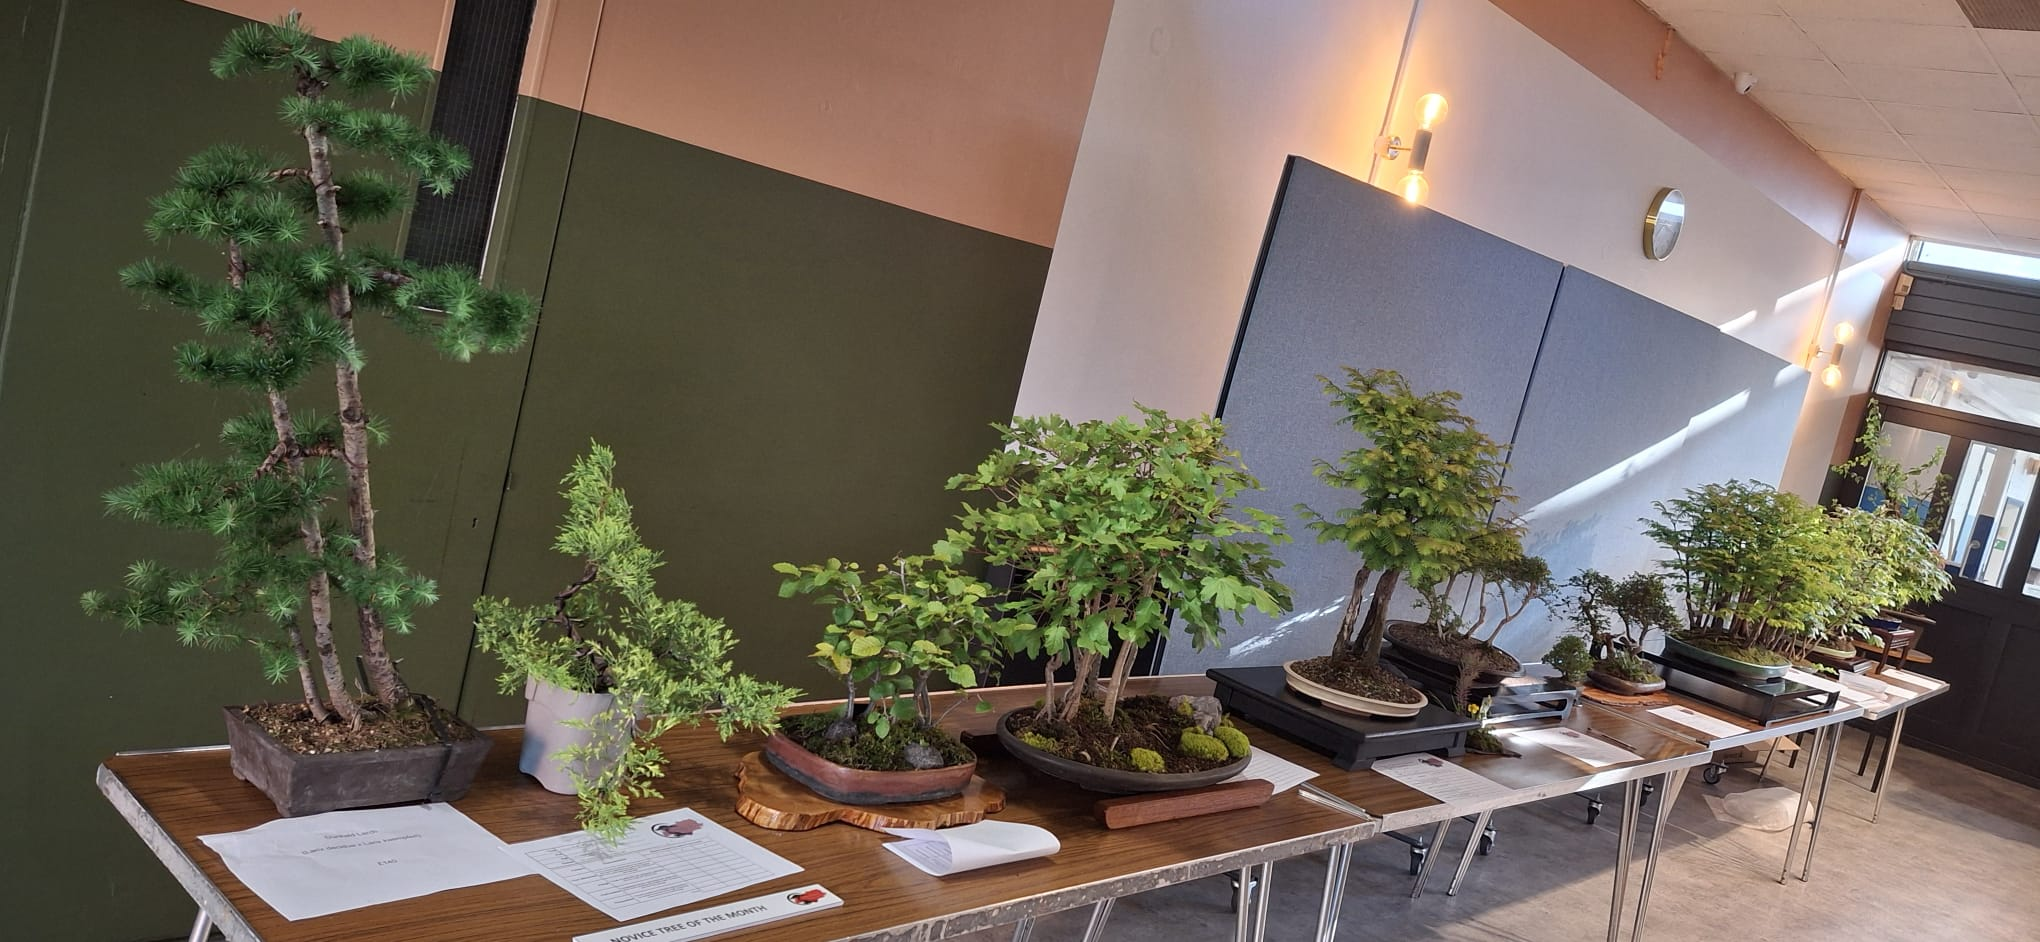
\includegraphics[width=1.0\textwidth]{2025_06/res/group_photo}
        \centerline{\emph{A forest of entries at June's meeting.}}
    \end{minipage}
\end{center}

\medskip
\begin{center}
    \begin{minipage}[b]{.4\textwidth}
        
\includegraphics[angle=0,origin=c,width=0.92\textwidth]{2025_06/res/contest_tree_01}
        % \centerline{\emph{David Fishwick's Cotoneaster.}}
    \end{minipage}\quad
    \begin{minipage}[b]{.4\textwidth}
        
\includegraphics[angle=0,origin=c,width=0.92\textwidth]{2025_06/res/contest_tree_02}
        % \centerline{\emph{Chris Durne's Cotoneaster.}}
    \end{minipage}

    \medskip
    \begin{minipage}[b]{.4\textwidth}
        
\includegraphics[angle=0,origin=c,width=0.92\textwidth]{2025_06/res/contest_tree_03}
        % \centerline{\emph{Brendan Gibbs' Cotoneaster.}}
    \end{minipage}\quad
    \begin{minipage}[b]{.4\textwidth}
        
\includegraphics[angle=0,origin=c,width=0.92\textwidth]{2025_06/res/contest_tree_04}
        % \centerline{\emph{Mark Pittman's Wisteria.}}
    \end{minipage}

    \medskip
    \centerline{\emph{Some of the trees that entered the Tree of the Month June contest.}}
\end{center}
\pagebreak

\begin{center}
    \begin{minipage}[b]{.4\textwidth}
        
\includegraphics[angle=0,origin=c,width=0.92\textwidth]{2025_06/res/contest_tree_05.jpeg}
        % \centerline{\emph{David Fishwick's Cotoneaster.}}
    \end{minipage}\quad
    \begin{minipage}[b]{.4\textwidth}
        
\includegraphics[angle=0,origin=c,width=0.92\textwidth]{2025_06/res/contest_tree_06.jpeg}
        % \centerline{\emph{Chris Durne's Cotoneaster.}}
    \end{minipage}

    \medskip
    \begin{minipage}[b]{.4\textwidth}
        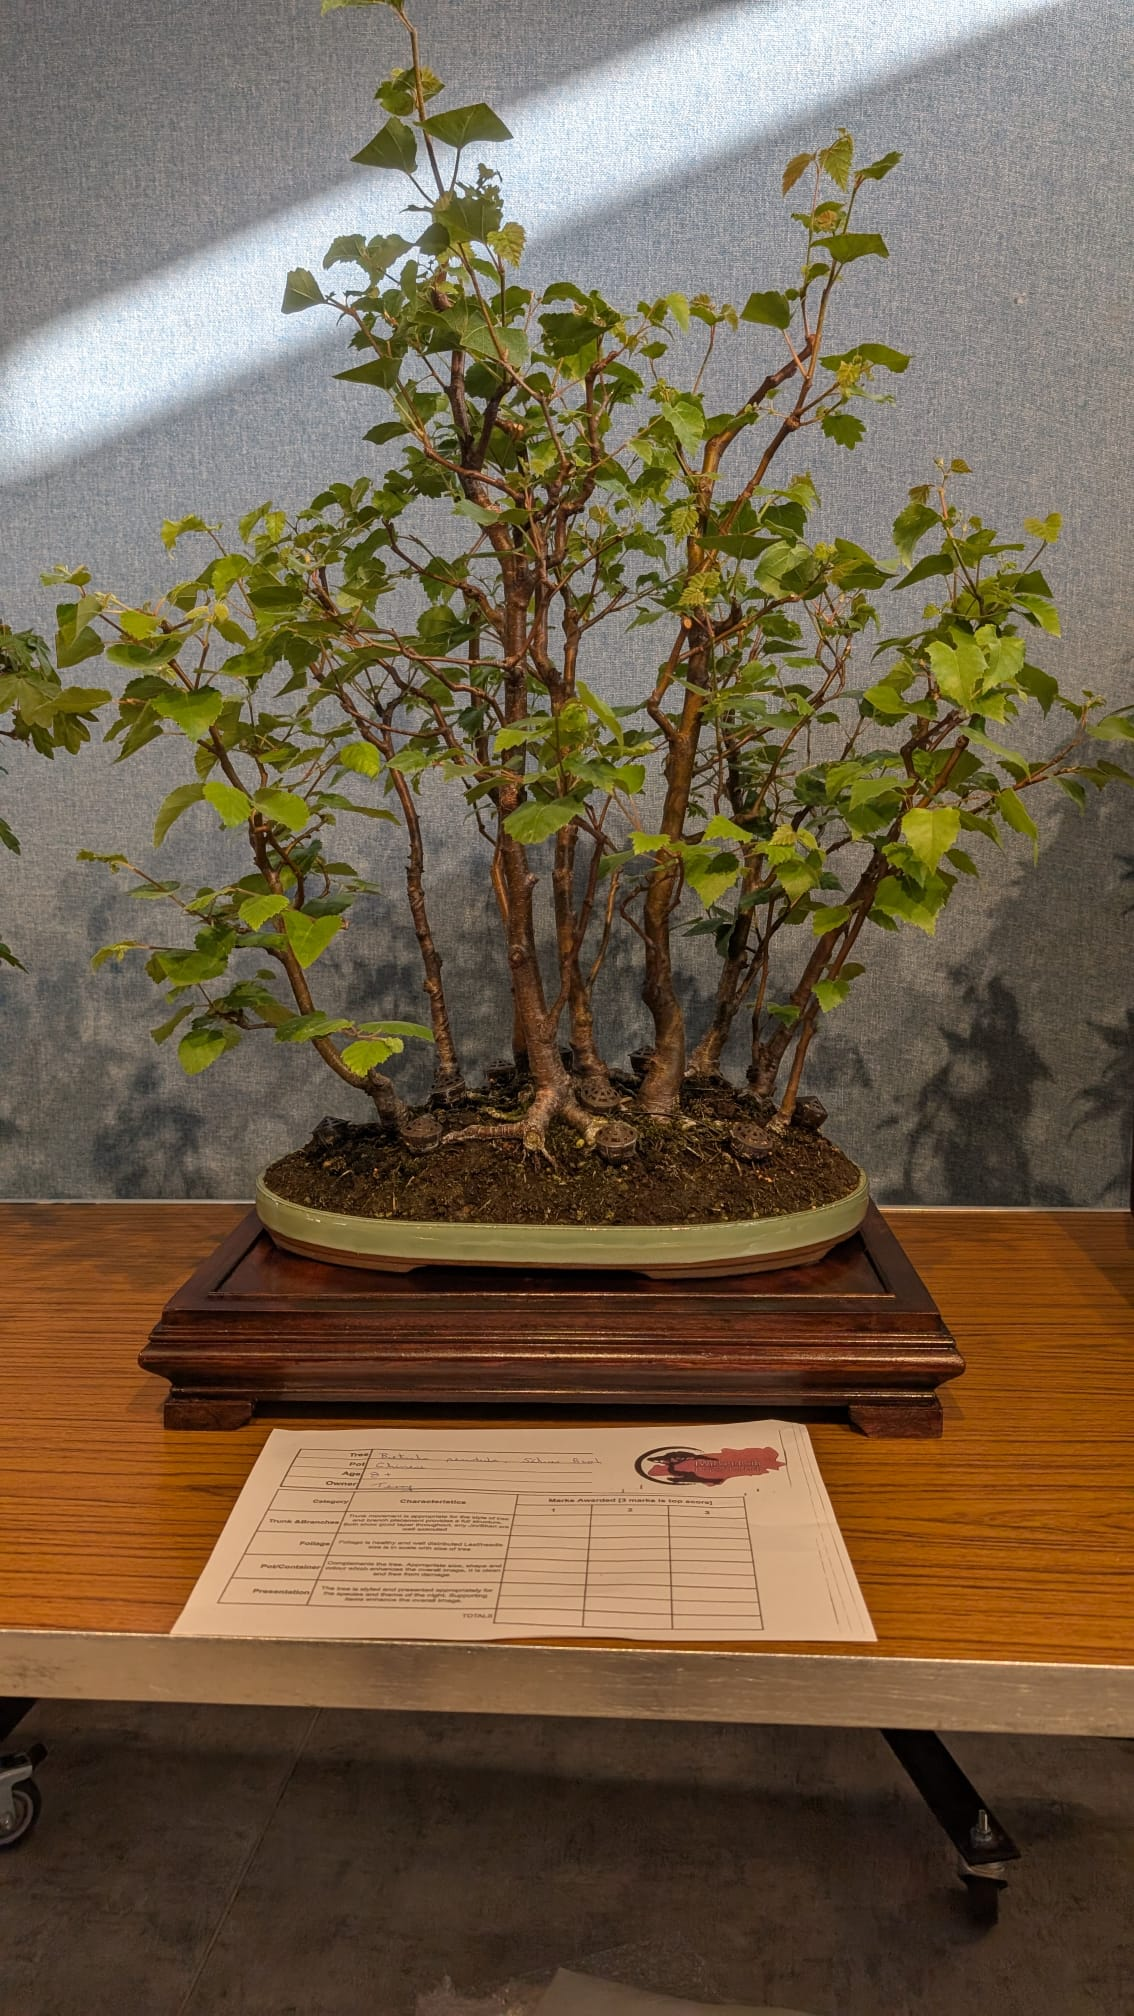
\includegraphics[angle=0,origin=c,width=0.92\textwidth]{2025_06/res/contest_tree_07.jpeg}
        % \centerline{\emph{Brendan Gibbs' Cotoneaster.}}
    \end{minipage}\quad
    \begin{minipage}[b]{.4\textwidth}
        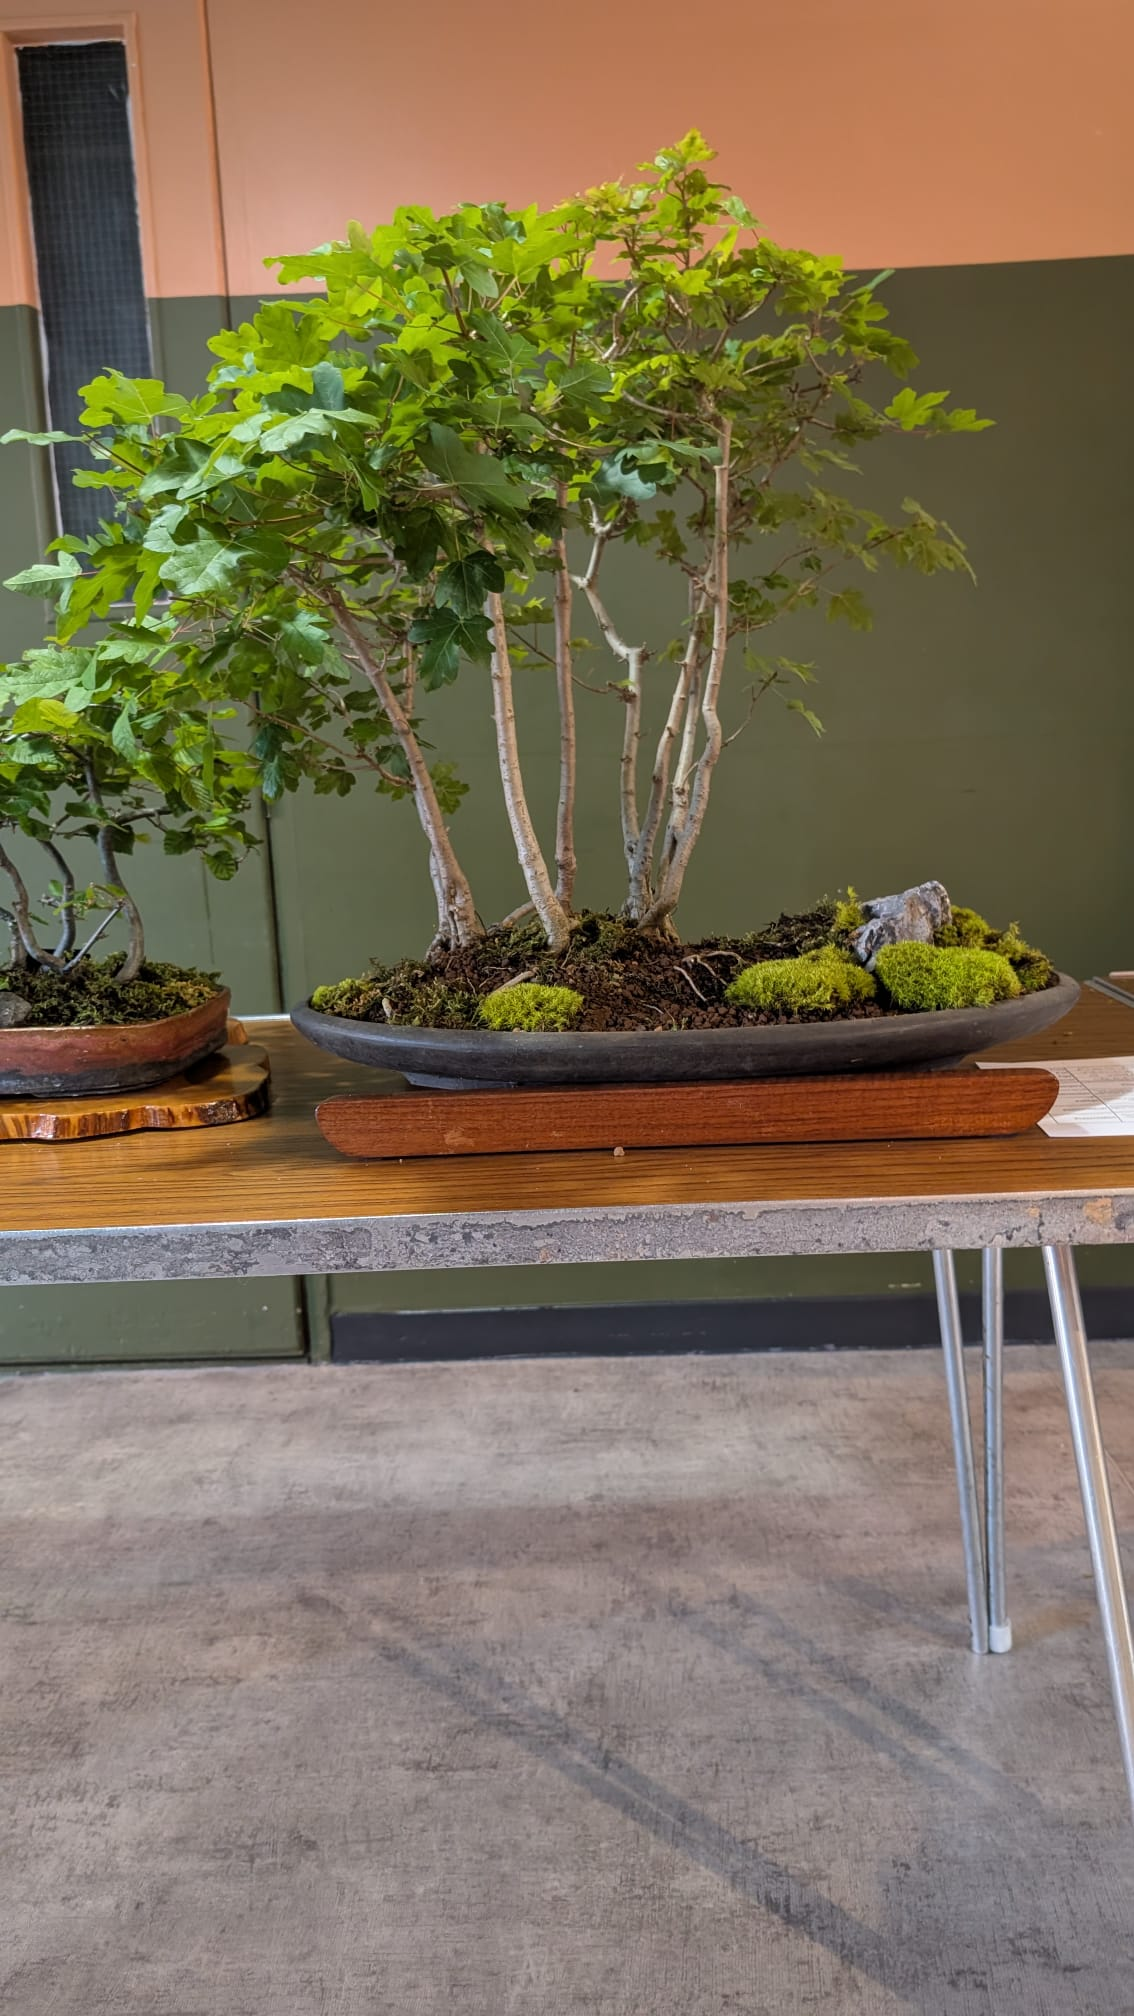
\includegraphics[angle=0,origin=c,width=0.92\textwidth]{2025_06/res/contest_tree_08.jpeg}
        % \centerline{\emph{Mark Pittman's Wisteria.}}
    \end{minipage}

    \medskip
    \centerline{\emph{Some of the trees that entered the Tree of the Month June contest.}}
\end{center}
\pagebreak

\begin{multicols}{2}
